% !TeX root = ../../../main.tex
\subsection{Experimental Results Details}
\label{ch02:sec:experimental-results-details}
\ChTwoHeadingOnly
\subsubsection{Synthetic Data Results}
\label{ch02:sec:ToyExperiment_Results}

In Figure~\ref{ch02:fig:toyDataset_result_complete}, we visualize the embedding space of all the models tested.
For all the baselines tested, we show the 3D embedding space.
For the \ChTwoSmallCaps{Temporal-SCL} model and its ablations where the embedding is constrained to lie on the hypersphere, we also plot the underlying unit hypersphere shell as well as the embeddings.


% !TeX root = ../../../main.tex
\begin{figure}[htbp]
\ChTwoFloatContents
    {ch02:fig:toyDataset_result_complete}%
    {\caption{Embedding space representation of the test trajectories of simulated dataset. For (a)- (j) 3D Embedding Space of baselines are shown which includes the purely supervised methods ((a)-(d)), predictive clustering methods ((e), (f)), and self-supervised learning methods ((g)-(j)). In (f)-(i), Hyperspherical Embedding of various ablated versions of \ChTwoSmallCaps{Temporal-SCL} is shown.}}%
    {%
        \subfigure[LSTM]{%
            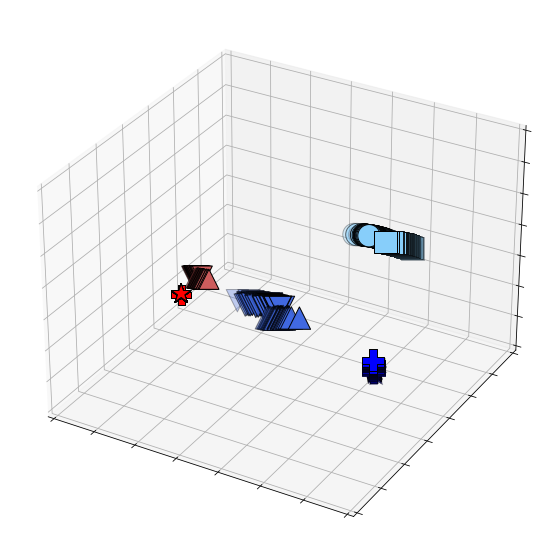
\includegraphics[width=0.21\textwidth]{Appendices/appendix-ch02/images/EmbeddingSpace_LSTM.png}
        }
        \subfigure[RETAIN]{%
            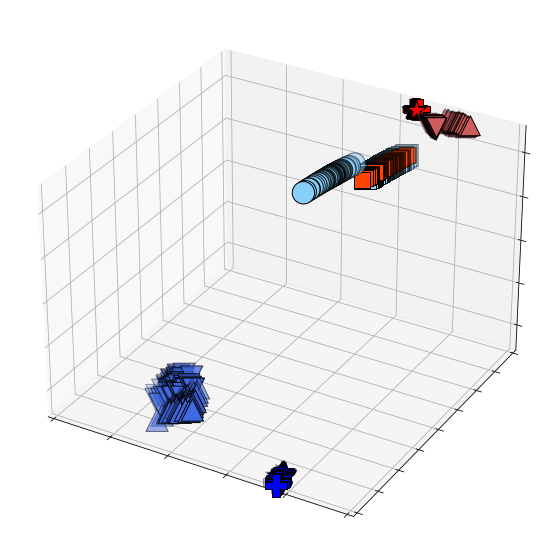
\includegraphics[width=0.21\textwidth]{Appendices/appendix-ch02/images/Embedding_RETAIN.png}
        }
        \subfigure[DIPOLE]{%
            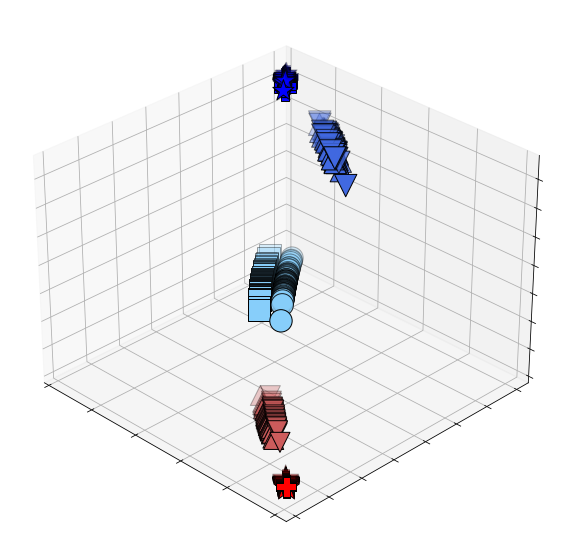
\includegraphics[width=0.21\textwidth]{Appendices/appendix-ch02/images/Embedding_DIPOLE.png}
        }
        \subfigure[Transformer]{%
            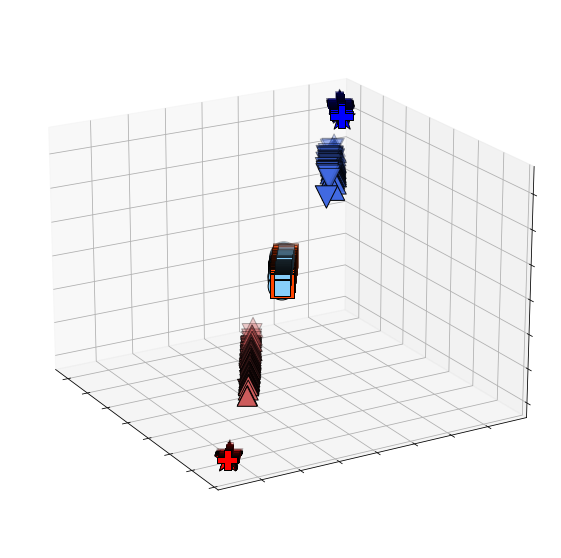
\includegraphics[width=0.21\textwidth]{Appendices/appendix-ch02/images/Embedding_Transformer.png}
        }\par\medskip
        \subfigure[AC-TPC]{%
            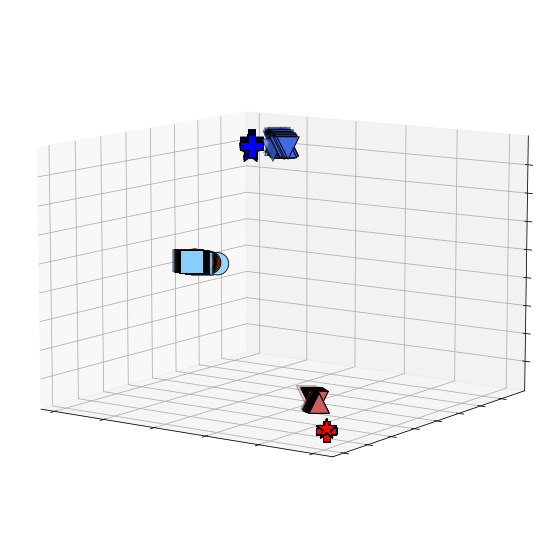
\includegraphics[width=0.21\textwidth]{Appendices/appendix-ch02/images/EmbeddingSpace_ACTPC.png}
        }
        \subfigure[T-Phenotype]{%
            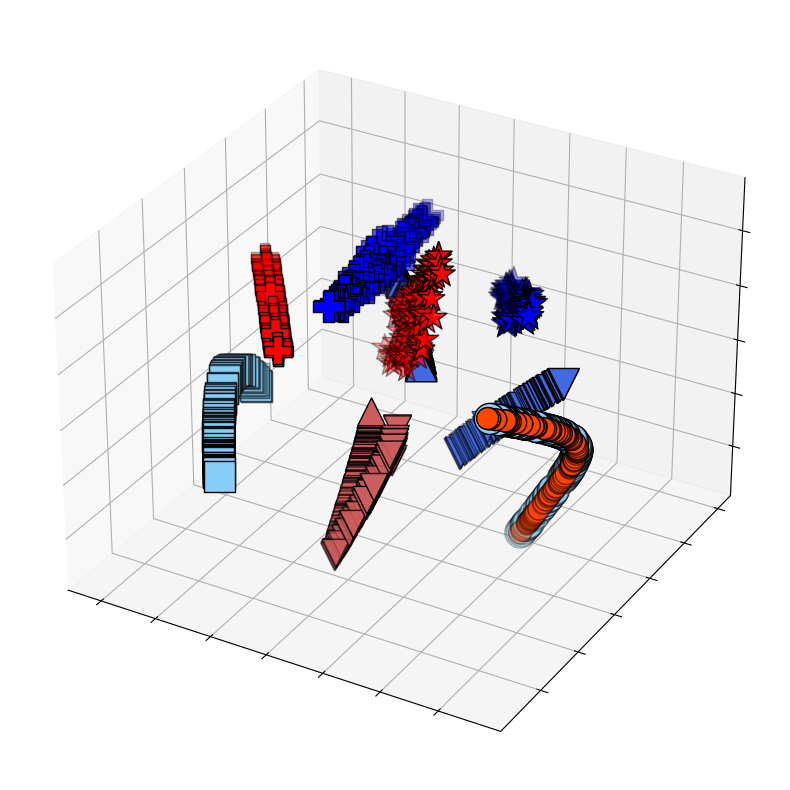
\includegraphics[width=0.21\textwidth]{Appendices/appendix-ch02/images/Embedding_TPhenotype.png}
        }
        \subfigure[SMD-SSL + SimCLR (Frozen)]{%
            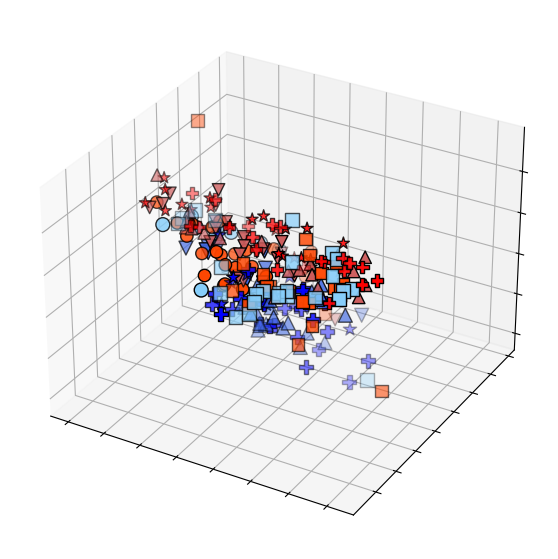
\includegraphics[width=0.21\textwidth]{Appendices/appendix-ch02/images/Embedding_SMDSSL_SimCLR_Freeze.png}
        }
        \subfigure[SMD-SSL + VICReg (Frozen)]{%
            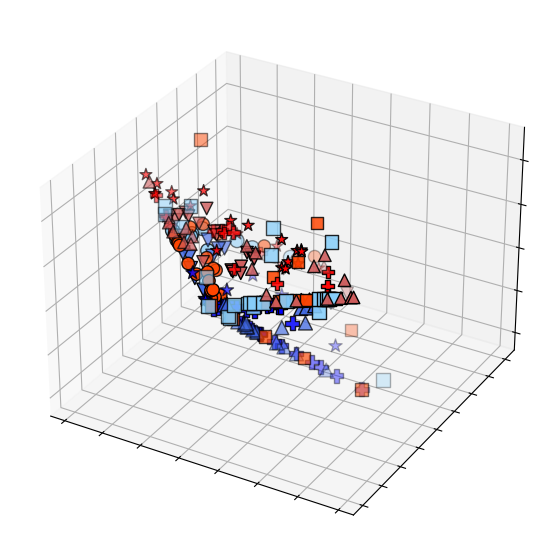
\includegraphics[width=0.21\textwidth]{Appendices/appendix-ch02/images/Embedding_SMDSSL_VICReg_Freeze.png}
        }\par\medskip
        \subfigure[SMD-SSL + SimCLR (Fine-tune)]{%
            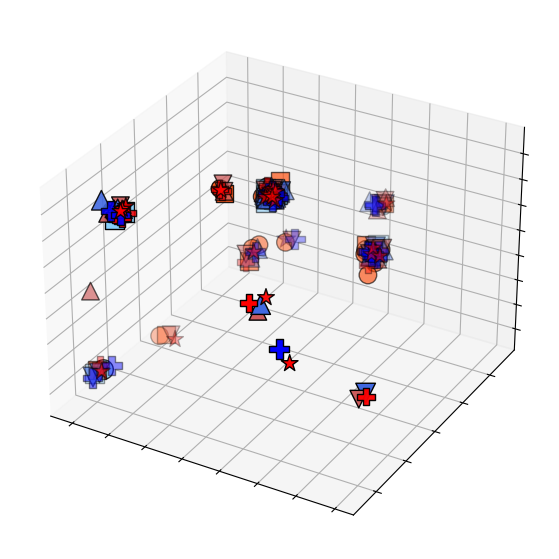
\includegraphics[width=0.21\textwidth]{Appendices/appendix-ch02/images/Embedding_SMDSSL_SimCLR.png}
        }
        \subfigure[SMD-SSL + VICReg (Fine-tune)]{%
            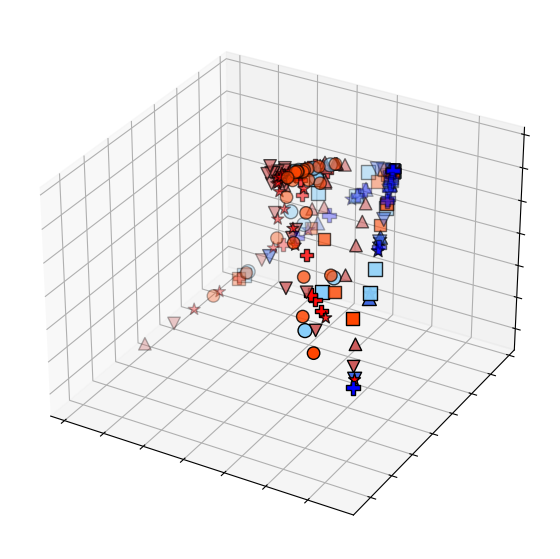
\includegraphics[width=0.21\textwidth]{Appendices/appendix-ch02/images/Embedding_SMDSSL_VICReg.png}
        }
        \subfigure[\ChTwoSmallCaps{Simple-SCL}]{%
            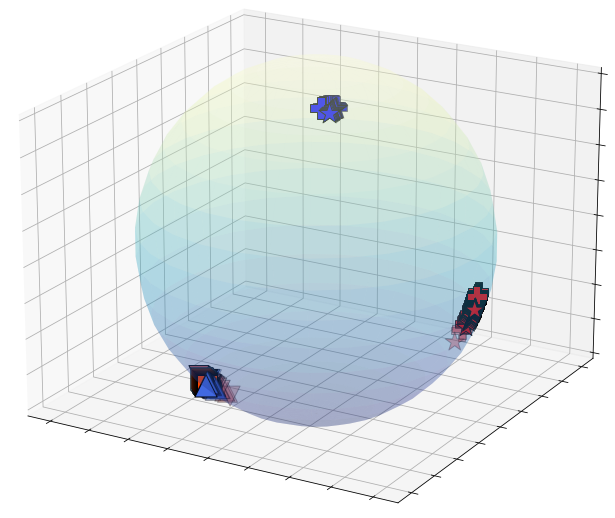
\includegraphics[width=0.21\textwidth]{Appendices/appendix-ch02/images/Embedding_SimpleSCL.png}
        }
        \subfigure[\ChTwoSmallCaps{Temporal-SCL} \newline no pretraining]{%
            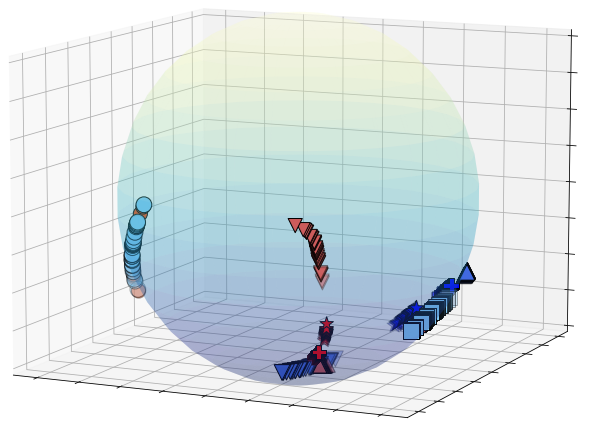
\includegraphics[width=0.21\textwidth]{Appendices/appendix-ch02/images/Embedding_NoPretrain.png}
        }\par\medskip
        \subfigure[\ChTwoSmallCaps{Temporal-SCL} \newline no NN pairing]{%
            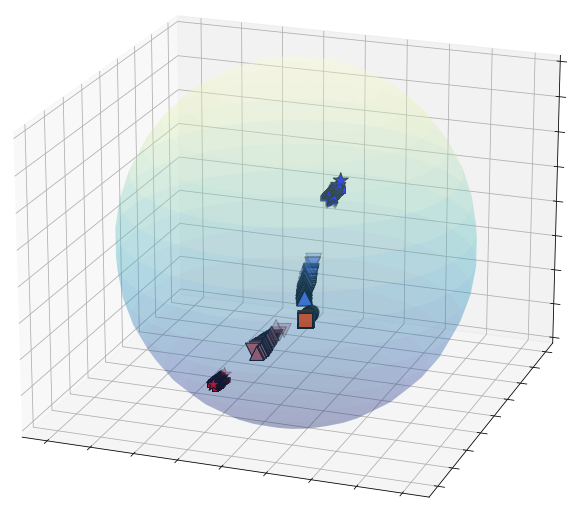
\includegraphics[width=0.21\textwidth]{Appendices/appendix-ch02/images/Embedding_NoKNN.png}
        }
        \subfigure[\ChTwoSmallCaps{Temporal-SCL}]{%
            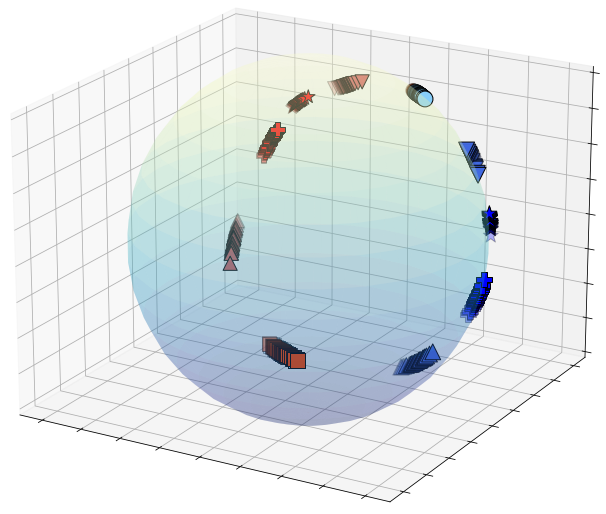
\includegraphics[width=0.21\textwidth]{Appendices/appendix-ch02/images/Embedding_TSCL.png}
        }
    }
\end{figure}


As it can be seen here, our proposed model is the only model that can fully recover the structure and the 10 clusters of time steps from the input raw feature space shown in Figure~\ref{ch02:fig:toyDataset_Raw}.

\subsubsection{Visualizing Embedding Clusters for MIMIC}
\label{ch02:sec:heatmap_mimic}
We show the full heatmap of Figure~\ref{ch02:fig:heatmapMIMIC} for how the features vary across clusters in the test set of our MIMIC dataset in Figure~\ref{ch02:fig:heatmapMIMIC_full}.
This heatmap is generated from the test patient embeddings of the complete \ChTwoSmallCaps{Temporal-SCL} model.
The heatmap uses the first version of our model out of the 10 experimental repeats.



\subsubsection{Visualizing Embedding Clusters for ADNI}
\label{ch02:sec:heatmap_adni}

To interpret each cluster for ADNI, we plot the heatmap how features (rows) vary across clusters for the test patients of ADNI in Figure \ref{ch02:fig:heatmapADNI}.
Columns are ordered (left to right) in dementia rate. 
Here we can also see that abnormal feature values that are correlated with higher risk of dementia such as irregular dementia rating scores are present in clusters containing higher proportion of AD.
The heatmap uses the first version of our model out of the 10 experimental repeats.




\subsubsection{Visualizing Embedding Clusters for MIMIC from Raw Features}
\label{ch02:sec:heatmap_mimic_raw}
We also tried our clustering-based heatmap visualization for clusters from raw feature vectors instead of \ChTwoSmallCaps{Temporal-SCL}’s embedding vectors.
Using raw features results in less useful heatmaps.
For example, in MIMIC as shown in Figure~\ref{ch02:fig:RawHeatmapADNI}, using raw feature vectors and 20 clusters, the resulting heatmap has high concentration in one cluster (93\% of data are in a single cluster) and the mortality rates across clusters are nearly all below 35\% (so the clusters found do not distinguish between patients with intermediate mortality probabilities, e.g., between 50\% to 100\%).
Neither of these issues arise when we cluster on our model’s embedding vectors as shown in Figure~\ref{ch02:fig:heatmapMIMIC_full}.



\subsubsection{Ablation Experiments}
\label{ch02:sec:ablation}

We conduct an ablation study of excluding the three modules of our framework: (1) pre-training, (2) nearest neighbor pairing, and (3) temporal network. 
Including or withholding each of these modules results in the following ablated models respectively:
\begin{enumerate}
    \item \ChTwoSmallCaps{Simple-SCL} \\(Pre-Training: \ChTwoXmark, NN Pairing: \ChTwoXmark, Temporal: \ChTwoXmark)
    \item \ChTwoSmallCaps{Temporal-SCL} - Pretrain Only \\ (Pre-Training: \ChTwoCmark, NN Pairing: \ChTwoXmark, Temporal: \ChTwoXmark)
    \item \ChTwoSmallCaps{Temporal-SCL} - NN Pairing Only \\ (Pre-Training: \ChTwoXmark, NN Pairing: \ChTwoCmark, Temporal: \ChTwoXmark)
    \item \ChTwoSmallCaps{Temporal-SCL} - Temporal Only \\ (Pre-Training: \ChTwoXmark, NN Pairing: \ChTwoXmark, Temporal: \ChTwoCmark)
    \item \ChTwoSmallCaps{Temporal-SCL} - No Pretrain \\ (Pre-Training: \ChTwoXmark, NN Pairing: \ChTwoCmark, Temporal: \ChTwoCmark)
    \item \ChTwoSmallCaps{Temporal-SCL} - No NN Pairing \\ (Pre-Training: \ChTwoCmark, NN Pairing: \ChTwoXmark, Temporal: \ChTwoCmark)
    \item \ChTwoSmallCaps{Temporal-SCL} - No Temporal \\ (Pre-Training: \ChTwoCmark, NN Pairing: \ChTwoCmark, Temporal: \ChTwoXmark)
    \item \ChTwoSmallCaps{Temporal-SCL} - Full \\ (Pre-Training: \ChTwoCmark, NN Pairing: \ChTwoCmark, Temporal: \ChTwoCmark)
\end{enumerate}
We observe that together, all three modules play a key role in performance for both our synthetic and real-world clinical datasets experiments. 


% !TeX root = ../../../main.tex
\begin{table}[ht!]
\caption{Ablation Study: Supervised and unsupervised performance.}
\setlength\tabcolsep{4pt}
\centering
\adjustbox{max width=\textwidth} {%
\begin{tabular}{cccccccc}
\toprule
\multirow{2}{*}[-2pt]{Dataset} &    \multirow{2}{*}[-2pt]{Model}    & \multicolumn{2}{c}{Supervised}                            & \multicolumn{4}{c}{Unsupervised} \\
                      \cmidrule(lr){3-4} \cmidrule(lr){5-8} %
                       &                                    & AUROC                      & AUPRC                    & Purity                    & NMI                       & ARI                       & SI \\ 
                       \midrule
                       \multirow{8}{*}{MIMIC}                      
                & \ChTwoSmallCaps{Simple-SCL} / \ChTwoSmallCaps{Temporal-SCL} (PT:\ChTwoXbmark, NN:\ChTwoXbmark, TR:\ChTwoXbmark)                       & 0.753$\pm$0.005          & 0.498$\pm$0.003            & 0.773$\pm$0.005           & 0.007$\pm$0.003           & 0.003$\pm$0.002           & 0.011$\pm$0.010 \\
                & \ChTwoSmallCaps{Temporal-SCL} (PT:\ChTwoCbmark, NN:\ChTwoXbmark, TR:\ChTwoXbmark)      & 0.752$\pm$0.002	       & 0.498$\pm$0.001	        & 0.770$\pm$0.005           & 0.006$\pm$0.003           & 0.002$\pm$0.002           & 0.011$\pm$0.001 \\ 
                & \ChTwoSmallCaps{Temporal-SCL} (PT:\ChTwoXbmark, NN:\ChTwoCbmark, TR:\ChTwoXbmark)   & 0.770$\pm$0.002	       & 0.516$\pm$0.003            & 0.788$\pm$0.002           & 0.093$\pm$0.006           & 0.108$\pm$0.031           & 0.269$\pm$0.021 \\
                & \ChTwoSmallCaps{Temporal-SCL} (PT:\ChTwoXbmark, NN:\ChTwoXbmark, TR:\ChTwoCbmark)      & 0.766$\pm$0.001	       & 0.508$\pm$0.002	        & 0.789$\pm$0.001           & 0.111$\pm$0.003           & 0.096$\pm$0.008           & 0.141$\pm$0.038 \\
                & \ChTwoSmallCaps{Temporal-SCL} (PT:\ChTwoXbmark, NN:\ChTwoCbmark, TR:\ChTwoCbmark)       & 0.754$\pm$0.006          & 0.499$\pm$0.003            & 0.775$\pm$0.000           & 0.007$\pm$0.002           & 0.002$\pm$0.001           & 0.031$\pm$0.018 \\
			& \ChTwoSmallCaps{Temporal-SCL} (PT:\ChTwoCbmark, NN:\ChTwoXbmark, TR:\ChTwoCbmark)      & 0.767$\pm$0.002          & 0.511$\pm$0.002            & 0.781$\pm$0.000           & 0.112$\pm$0.007           & {\ChTwoBfTab 0.150$\pm$0.034}  & 0.143$\pm$0.007 \\ 
                & \ChTwoSmallCaps{Temporal-SCL} (PT:\ChTwoCbmark, NN:\ChTwoCbmark, TR:\ChTwoXbmark)        & 0.770$\pm$0.002	       & 0.518$\pm$0.003	        & 0.776$\pm$0.001           & 0.091$\pm$0.004           & 0.097$\pm$0.009           & 0.398$\pm$0.055 \\
                & \ChTwoSmallCaps{Temporal-SCL} (Full)              & {\ChTwoBfTab 0.773$\pm$0.002} &{\ChTwoBfTab 0.520$\pm$0.003}    & {\ChTwoBfTab 0.793$\pm$0.001}  & {\ChTwoBfTab 0.115$\pm$0.002}  & 0.128$\pm$0.014           & {\ChTwoBfTab 0.423$\pm$0.065} \\ 
                       \midrule
\multirow{8}{*}{ADNI}  
                & \ChTwoSmallCaps{Simple-SCL} / \ChTwoSmallCaps{Temporal-SCL} (PT:\ChTwoXbmark, NN:\ChTwoXbmark, TR:\ChTwoXbmark)                        & 0.947$\pm$0.001          & 0.894$\pm$0.015            & 0.639$\pm$0.023           & 0.159$\pm$0.058           & 0.230$\pm$0.012           & 0.177$\pm$0.144   \\
                & \ChTwoSmallCaps{Temporal-SCL} (PT:\ChTwoCbmark, NN:\ChTwoXbmark, TR:\ChTwoXbmark)      & 0.947$\pm$0.001	       & 0.894$\pm$0.014	        & 0.640$\pm$0.029           & 0.163$\pm$0.042           & 0.219$\pm$0.018           & 0.176$\pm$0.150 \\
                & \ChTwoSmallCaps{Temporal-SCL} (PT:\ChTwoXbmark, NN:\ChTwoCbmark, TR:\ChTwoXbmark)   & 0.987$\pm$0.001	       & 0.899$\pm$0.011	        & 0.753$\pm$0.010           & 0.408$\pm$0.026           & 0.288$\pm$0.017           & 0.199$\pm$0.029 \\
                & \ChTwoSmallCaps{Temporal-SCL} (PT:\ChTwoXbmark, NN:\ChTwoXbmark, TR:\ChTwoCbmark)      & 0.950$\pm$0.002	       & 0.785$\pm$0.015	        & 0.685$\pm$0.025           & 0.262$\pm$0.016           & 0.210$\pm$0.071           & 0.159$\pm$0.101 \\           
                & \ChTwoSmallCaps{Temporal-SCL} (PT:\ChTwoXbmark, NN:\ChTwoCbmark, TR:\ChTwoCbmark)        & 0.967$\pm$0.002          & 0.900$\pm$0.017            & 0.713$\pm$0.095           & 0.275$\pm$0.120           & 0.209$\pm$0.104           & 0.149$\pm$0.080 \\ 
			& \ChTwoSmallCaps{Temporal-SCL} (PT:\ChTwoCbmark, NN:\ChTwoXbmark, TR:\ChTwoCbmark)      & 0.951$\pm$0.002          & 0.762$\pm$0.010            & 0.749$\pm$0.009           & 0.446$\pm$0.009           & 0.334$\pm$0.015           & 0.163$\pm$0.008 \\ 
                & \ChTwoSmallCaps{Temporal-SCL} (PT:\ChTwoCbmark, NN:\ChTwoCbmark, TR:\ChTwoXbmark)        & 0.988$\pm$0.001	       & 0.903$\pm$0.011	        & 0.753$\pm$0.011           & 0.415$\pm$0.024           & 0.300$\pm$0.042           & 0.197$\pm$0.033 \\
                & \ChTwoSmallCaps{Temporal-SCL} (Full)              & {\ChTwoBfTab 0.990$\pm$0.004} & {\ChTwoBfTab 0.936$\pm$0.014}   & {\ChTwoBfTab 0.755$\pm$0.023}  & {\ChTwoBfTab 0.452$\pm$0.031}  & {\ChTwoBfTab 0.399$\pm$0.010}  & {\ChTwoBfTab 0.259$\pm$0.031} \\
\bottomrule
\end{tabular}}


{\scriptsize {\ChTwoBfTab{PT}}: Pre-Training, {\ChTwoBfTab{NN}}: Nearest Neighbor pairing, {\ChTwoBfTab{TR}}: Temporal Regularization\\}
\ChTwoFloatLabel{ch02:tab:ablation_results}
\end{table}


\textbf{Synthetic dataset.} 
In Table~\ref{ch02:tab:toyDataset_ratios}, examining the ablated models reveals the distinct contributions of each module in our synthetic experiments.
Specifically, the observed decrease in Silhouette Index (SI) when NN pairing is absent underscores its pivotal role in maintaining feature similarity, which is instrumental in ground truth recovery.
Conversely, the model lacking pre-training suggests that while pre-training facilitates initial model configuration, the presence of NN pairing and the temporal network can partly mitigate its absence.

These results highlight the NN pairing module's significance in organizing the embedding space, a notion further evidenced by the relatively higher SI in the NN Pairing Only ablation (3) compared to other single-module ablations.

The temporal network's role, while not markedly influencing performance metrics in isolation, proves vital for the temporal structure within the embedding space.
This is contrasted with the \ChTwoSmallCaps{Simple-SCL} model, where the simultaneous absence of NN pairing and the temporal network leads to the lowest performance metrics, emphasizing the necessity of their collective functionality.

The full \ChTwoSmallCaps{Temporal-SCL} configuration exhibits superior SI and Cluster Prediction Accuracy, demonstrating the synergistic effect of the three modules in both the recovery of input structure and the enhancement of downstream task prediction.

In Figure~\ref{ch02:fig:toyDataset_result_complete}, we include ablations of the most simple model (1) and ablations of single module omitted (6), (7), alongside the fully-equipped model (8).
The learned embedding space from these models illustrates high prediction accuracy, as evidenced by a hyperplane nearly perfectly segregating the red data points from the blue data points.
However, the figure also showcases the collective capacity of the modules to recover the known ground-truth embedding vectors.
Notably, only the complete model represented in Figure~\ref{ch02:fig:synth-tscl} achieves an accurate reconstruction of the embedding structure, evidenced by distinct, correctly ordered clusters for each timestep.


\noindent
\textbf{Clinical datasets.} We present an ablation study of our model to see how each modification contributes to the performance.
Our full model includes pre-training with \ChTwoSmallCaps{Simple-SCL}, enhancing the Temporal Network $h$, and using ``labels$+$feature-similarity'' for finding the nearest neighbor pairs. 
We train the extra 7 additional ablated models in this section on both our MIMIC and ADNI datasets.
Note that to discover discrete latent states that could be of interest, we cluster on the learned hyperspherical embeddings (the $\mathbf{z}_i^{(\ell)}$ variables)  using a complete linkage Agglomerative Hierarchical Clustering \citep{murtagh2012algorithms}.
We describe our clustering approach in Appendix~\ref{ch02:sec:cluster}.
The unsupervised metrics presented here are evaluated for the same number of clusters in each ablation.


% !TeX root = ../../../main.tex
\begin{table}[ht!]
\caption{Future Prediction on ADNI data test set accuracy (mean $\pm$ std.~dev.~across 10 experiments).}
\centering
\setlength\tabcolsep{8pt}
\scriptsize
\begin{tabular}{ccccc} 
\toprule
		\multirow{2}{*}[-2pt]{Model}                                       & \multicolumn{2}{c}{6 months in the future}                          & \multicolumn{2}{c}{1 year in the future}                                                   \\ \cmidrule(lr){2-3} \cmidrule(lr){4-5} %
                                                               & AUROC                    & AUPRC                   & AUROC                   & AUPRC \\ 
                       \midrule  %
                        Logistic Regression                    & 0.825$\pm$0.007          & 0.659$\pm$0.008         & 0.767$\pm$0.006          & 0.620$\pm$0.012 \\
					  LSTM                                   & \text{0.880$\pm$0.003}   & 0.789$\pm$0.005         & 0.856$\pm$0.004          & 0.736$\pm$0.008 \\
                        RETAIN                                 & \text{0.882$\pm$0.010}   & 0.793$\pm$0.016         & \text{0.867$\pm$0.013}   & 0.740$\pm$0.017 \\
                        DIPOLE                                 & \text{0.940$\pm$0.006}   & 0.864$\pm$0.009         & \text{0.918$\pm$0.008}   & 0.813$\pm$0.010 \\
                        AC-TPC                                 & 0.823$\pm$0.011          & 0.702$\pm$0.016         & 0.804$\pm$0.014          & 0.679$\pm$0.020 \\
                        Transformer:BERT                       & \text{0.947$\pm$0.005}   & 0.880$\pm$0.010         & \text{0.939$\pm$0.007}   & \text{0.846$\pm$0.011} \\
                        \cmidrule(lr){1-5}
                        \ChTwoSmallCaps{Simple-SCL}                    & 0.922$\pm$0.005          & 0.794$\pm$0.016         & 0.899$\pm$0.003          & 0.764$\pm$0.015    \\
                        \ChTwoSmallCaps{Temporal-SCL} (PT:\ChTwoXbmark, NN:\ChTwoCbmark, TR:\ChTwoCbmark)    & 0.950$\pm$0.002          & {0.878$\pm$0.014}       & 0.930$\pm$0.002          & {0.807$\pm$0.018}  \\ 
					 \ChTwoSmallCaps{Temporal-SCL} (PT:\ChTwoCbmark, NN:\ChTwoXbmark, TR:\ChTwoCbmark)    & 0.948$\pm$0.002          & {0.842$\pm$0.012}       & 0.929$\pm$0.002          & {0.800$\pm$0.011}  \\ 
                       \ChTwoSmallCaps{Temporal-SCL} (Full)            & {\ChTwoBfTab 0.985$\pm$0.002} &{\ChTwoBfTab 0.907$\pm$0.012} & {\ChTwoBfTab 0.970$\pm$0.003} & {\ChTwoBfTab 0.878$\pm$0.015}  \\ 
\bottomrule
\end{tabular}


{\scriptsize {\ChTwoBfTab{PT}}: Pre-Training, {\ChTwoBfTab{NN}}: Nearest Neighbor pairing, {\ChTwoBfTab{TR}}: Temporal Regularization\\}
\ChTwoFloatLabel{ch02:tab:results_future_adni}
\end{table}


Firstly, our empirical findings show that for the models without pre-training and without the temporal network $h$ (\ChTwoSmallCaps{Simple-SCL}), we see a clear performance drop for all supervised and unsupervised metrics which highlights the importance of inclusion of these modules in our model training.
We also calculated the Silhouette Index (SI) of the ablated models in the last column of Table~\ref{ch02:tab:ablation_results}.
As it can be seen from the ablation results, with respect to the supervised prediction performance (AUROC, AUPRC), the two models with and without NN pairing ((5), (8)) perform similarly.
However, the main gain of using “labels+feature similarity” comes in the unsupervised prediction performance (Purity, NMI, ARI, SI).
This is especially apparent in the Silhouette Index score (a measure of how similar an object is to its own cluster compared to other clusters) where we see the greatest boost in performance when using “labels+feature similarity” (full model (8)) instead of “labels only” (ablated model (5)) where it shows how our model moves away from just stratifying risk (which is what the supervised metrics are measuring) to additionally being capable of identifying homogeneous disease phenotypes.
These experiments together, underscore the significance of having the different building blocks of our model for achieving the highest performance gain in our experiments.

Additionally, the ablation results shown in the bottom portion of Table~\ref{ch02:tab:results} reveal that the highest performance gain with respect to the supervised prediction performance (AUROC, AUPRC) is achieved by the full \ChTwoSmallCaps{Temporal-SCL}.
In our MIMIC experiment, the ablated model without only the nearest neighbor pairing achieves the closest performance to the full model, while in ADNI, where the prediction task seems to be easier (as evident by the high prediction scores), the ablated model without pre-training and the ablated model without the temporal regularization of our temporal network are the closests to the full model with respect to the prediction performance.
These experiments again underscore the significance of the different building blocks of our model to achieve the greatest performance gain in our experiments within MIMIC and ADNI datasets.

\subsubsection{Additional Experiments on ADNI: Predicting Future Cognitive Impairment Status}
\label{ch02:sec:future_adni}
In our experiments presented in \ref{ch02:sec:ClinicalExperiments}, we followed the same experimental paradigm of predicting the current time step label as conducted by \cite{lee2020temporal}. 
In this section however we will look at an additional prediction task for predicting the cognitive impairment 6 months and 1 year in the future. 
The results are presented in Table~\ref{ch02:tab:results_future_adni} below. 
We can see that for this prediction task again our model outperforms other baselines.


% !TeX root = ../../../main.tex
\begin{figure}[t!]
\centering
 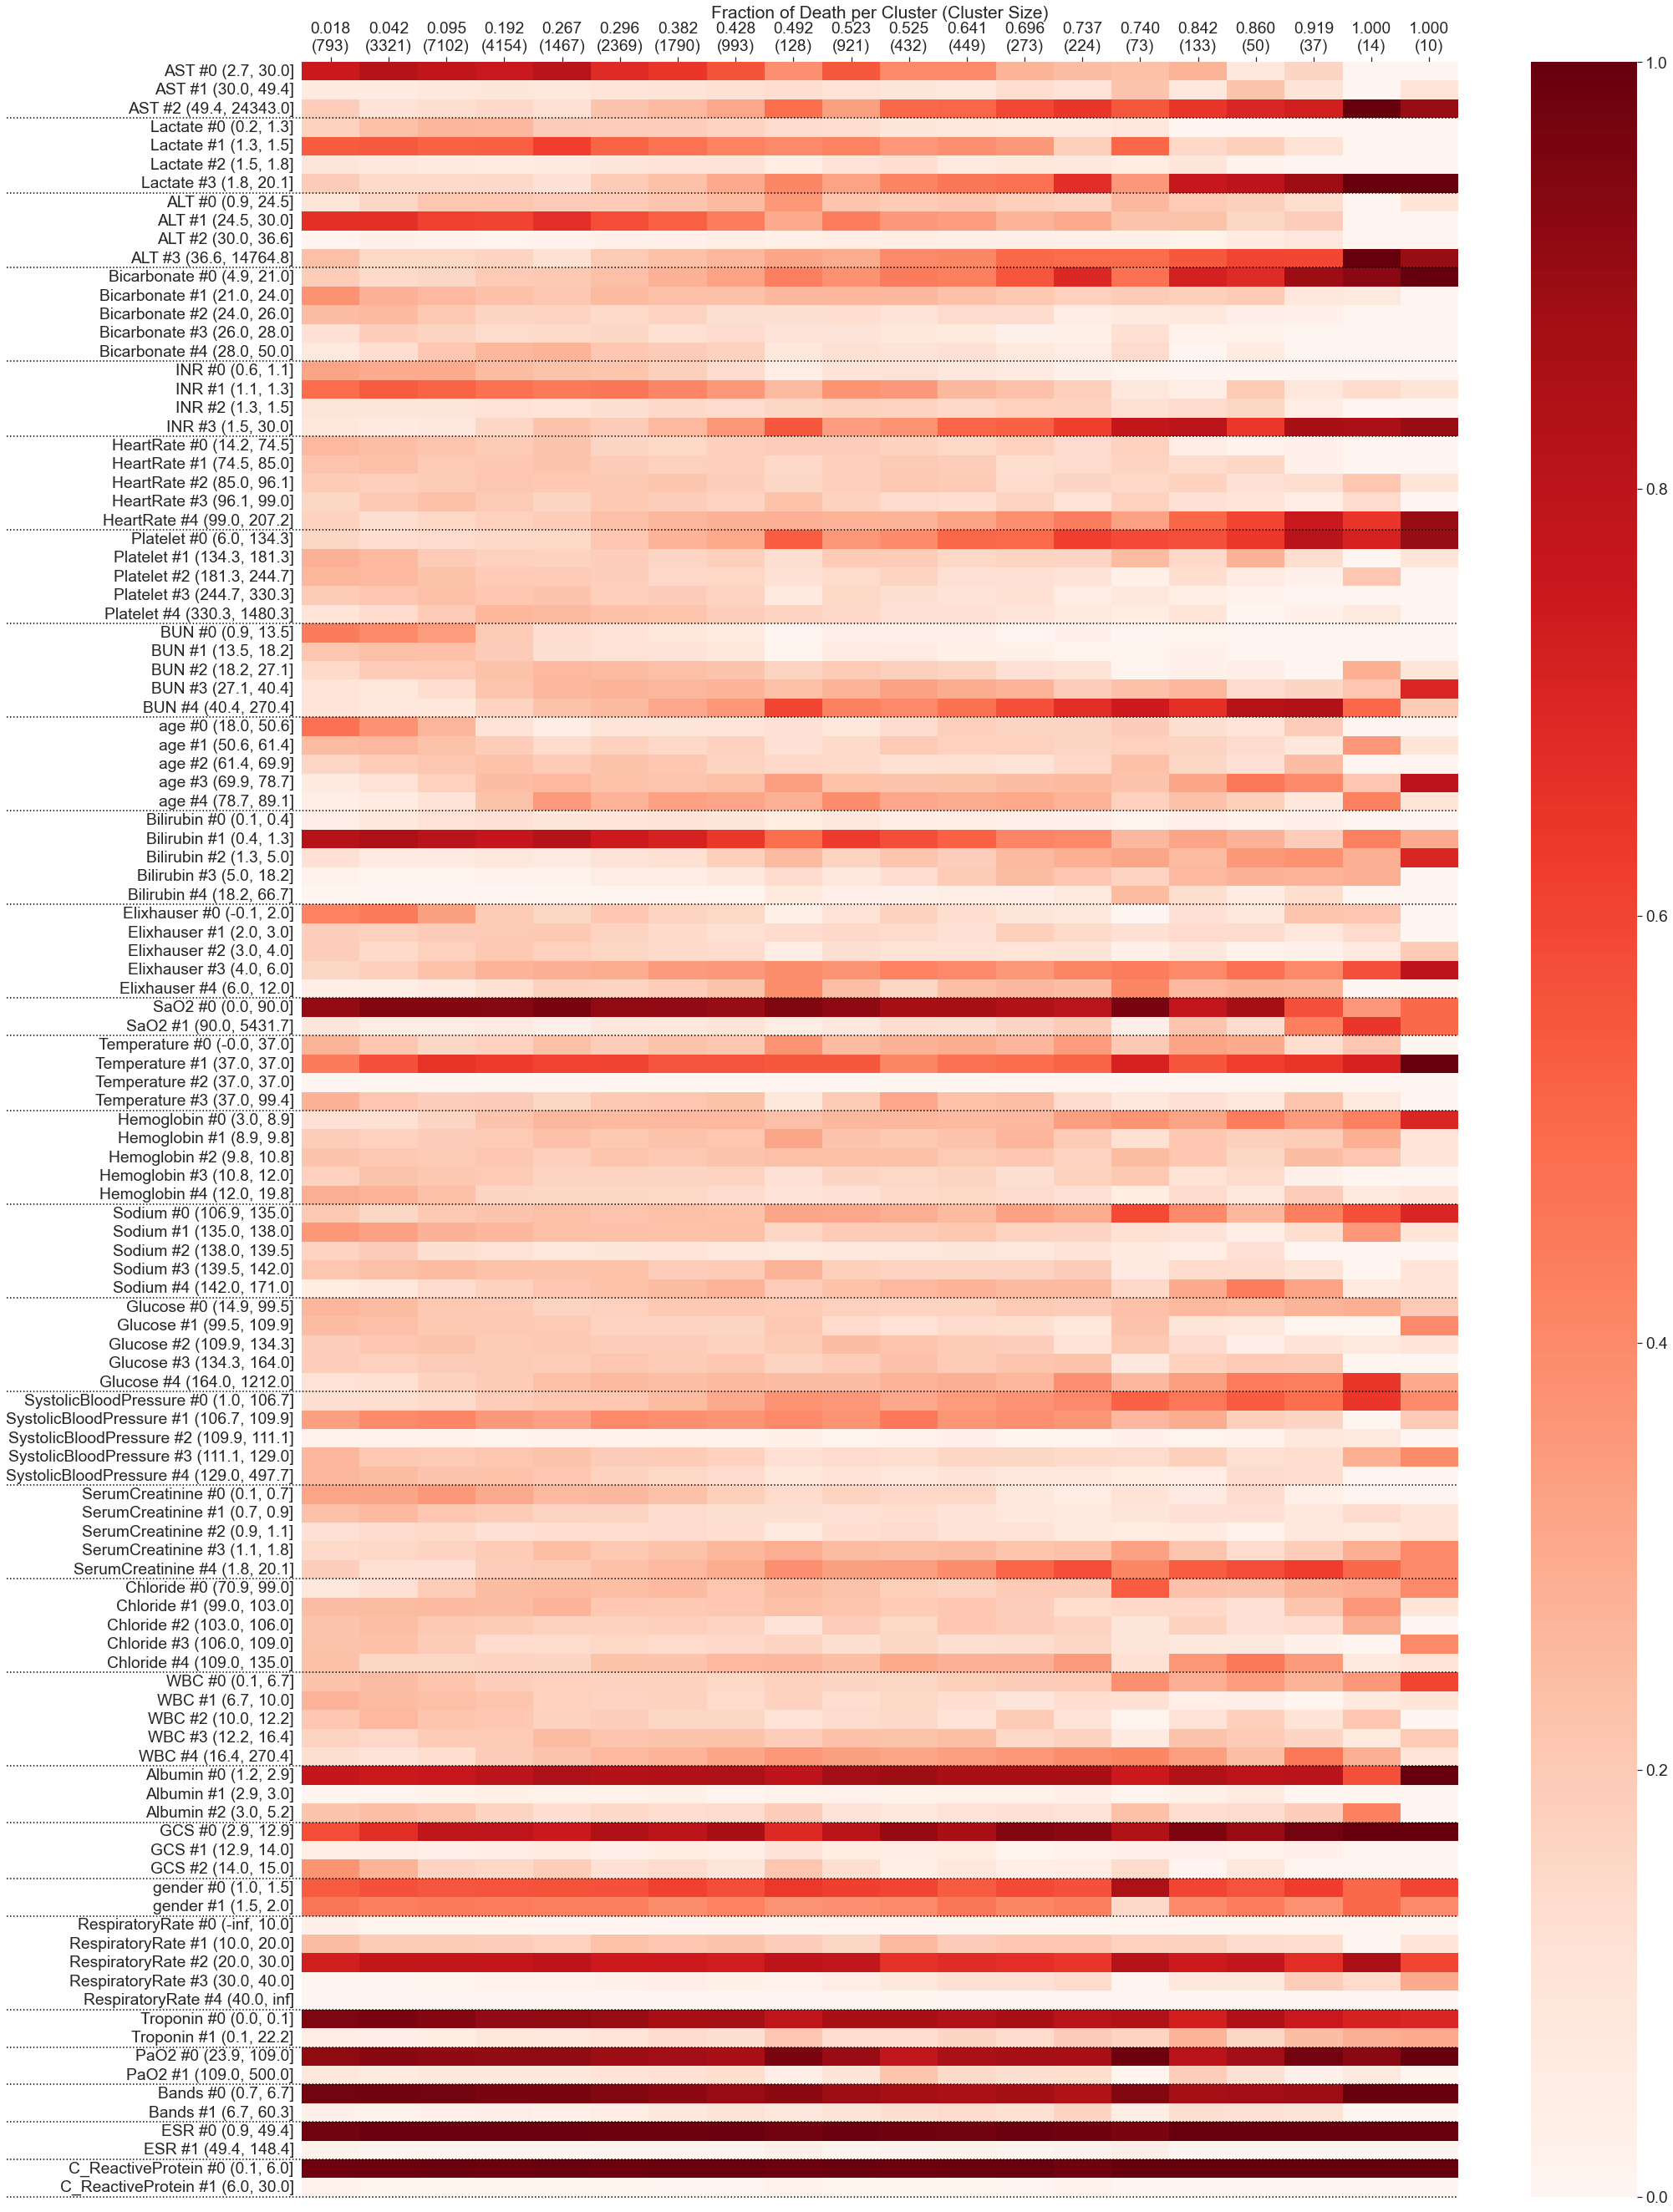
\includegraphics[width=.9\linewidth,height=0.68\textheight,keepaspectratio]{Appendices/appendix-ch02/images/mimicHeatmapFull.png}
 
  \caption{Heatmap showing how features (rows) vary across clusters (columns) for the sepsis cohort of the MIMIC dataset when using \emph{clustering on \ChTwoSmallCaps{Temporal-SCL} learned embedding space}. Heatmap intensity values can be thought of as the conditional probability of seeing a feature value (row) conditioned on being in a cluster (column); these probabilities are estimated using test set snapshots. Columns are ordered left to right in increasing fraction of test set snapshots that come from a time series that has a final outcome of death.
 }
    \ChTwoFloatLabel{ch02:fig:heatmapMIMIC_full}  
\end{figure}



% !TeX root = ../../../main.tex
\begin{figure}[t!]
 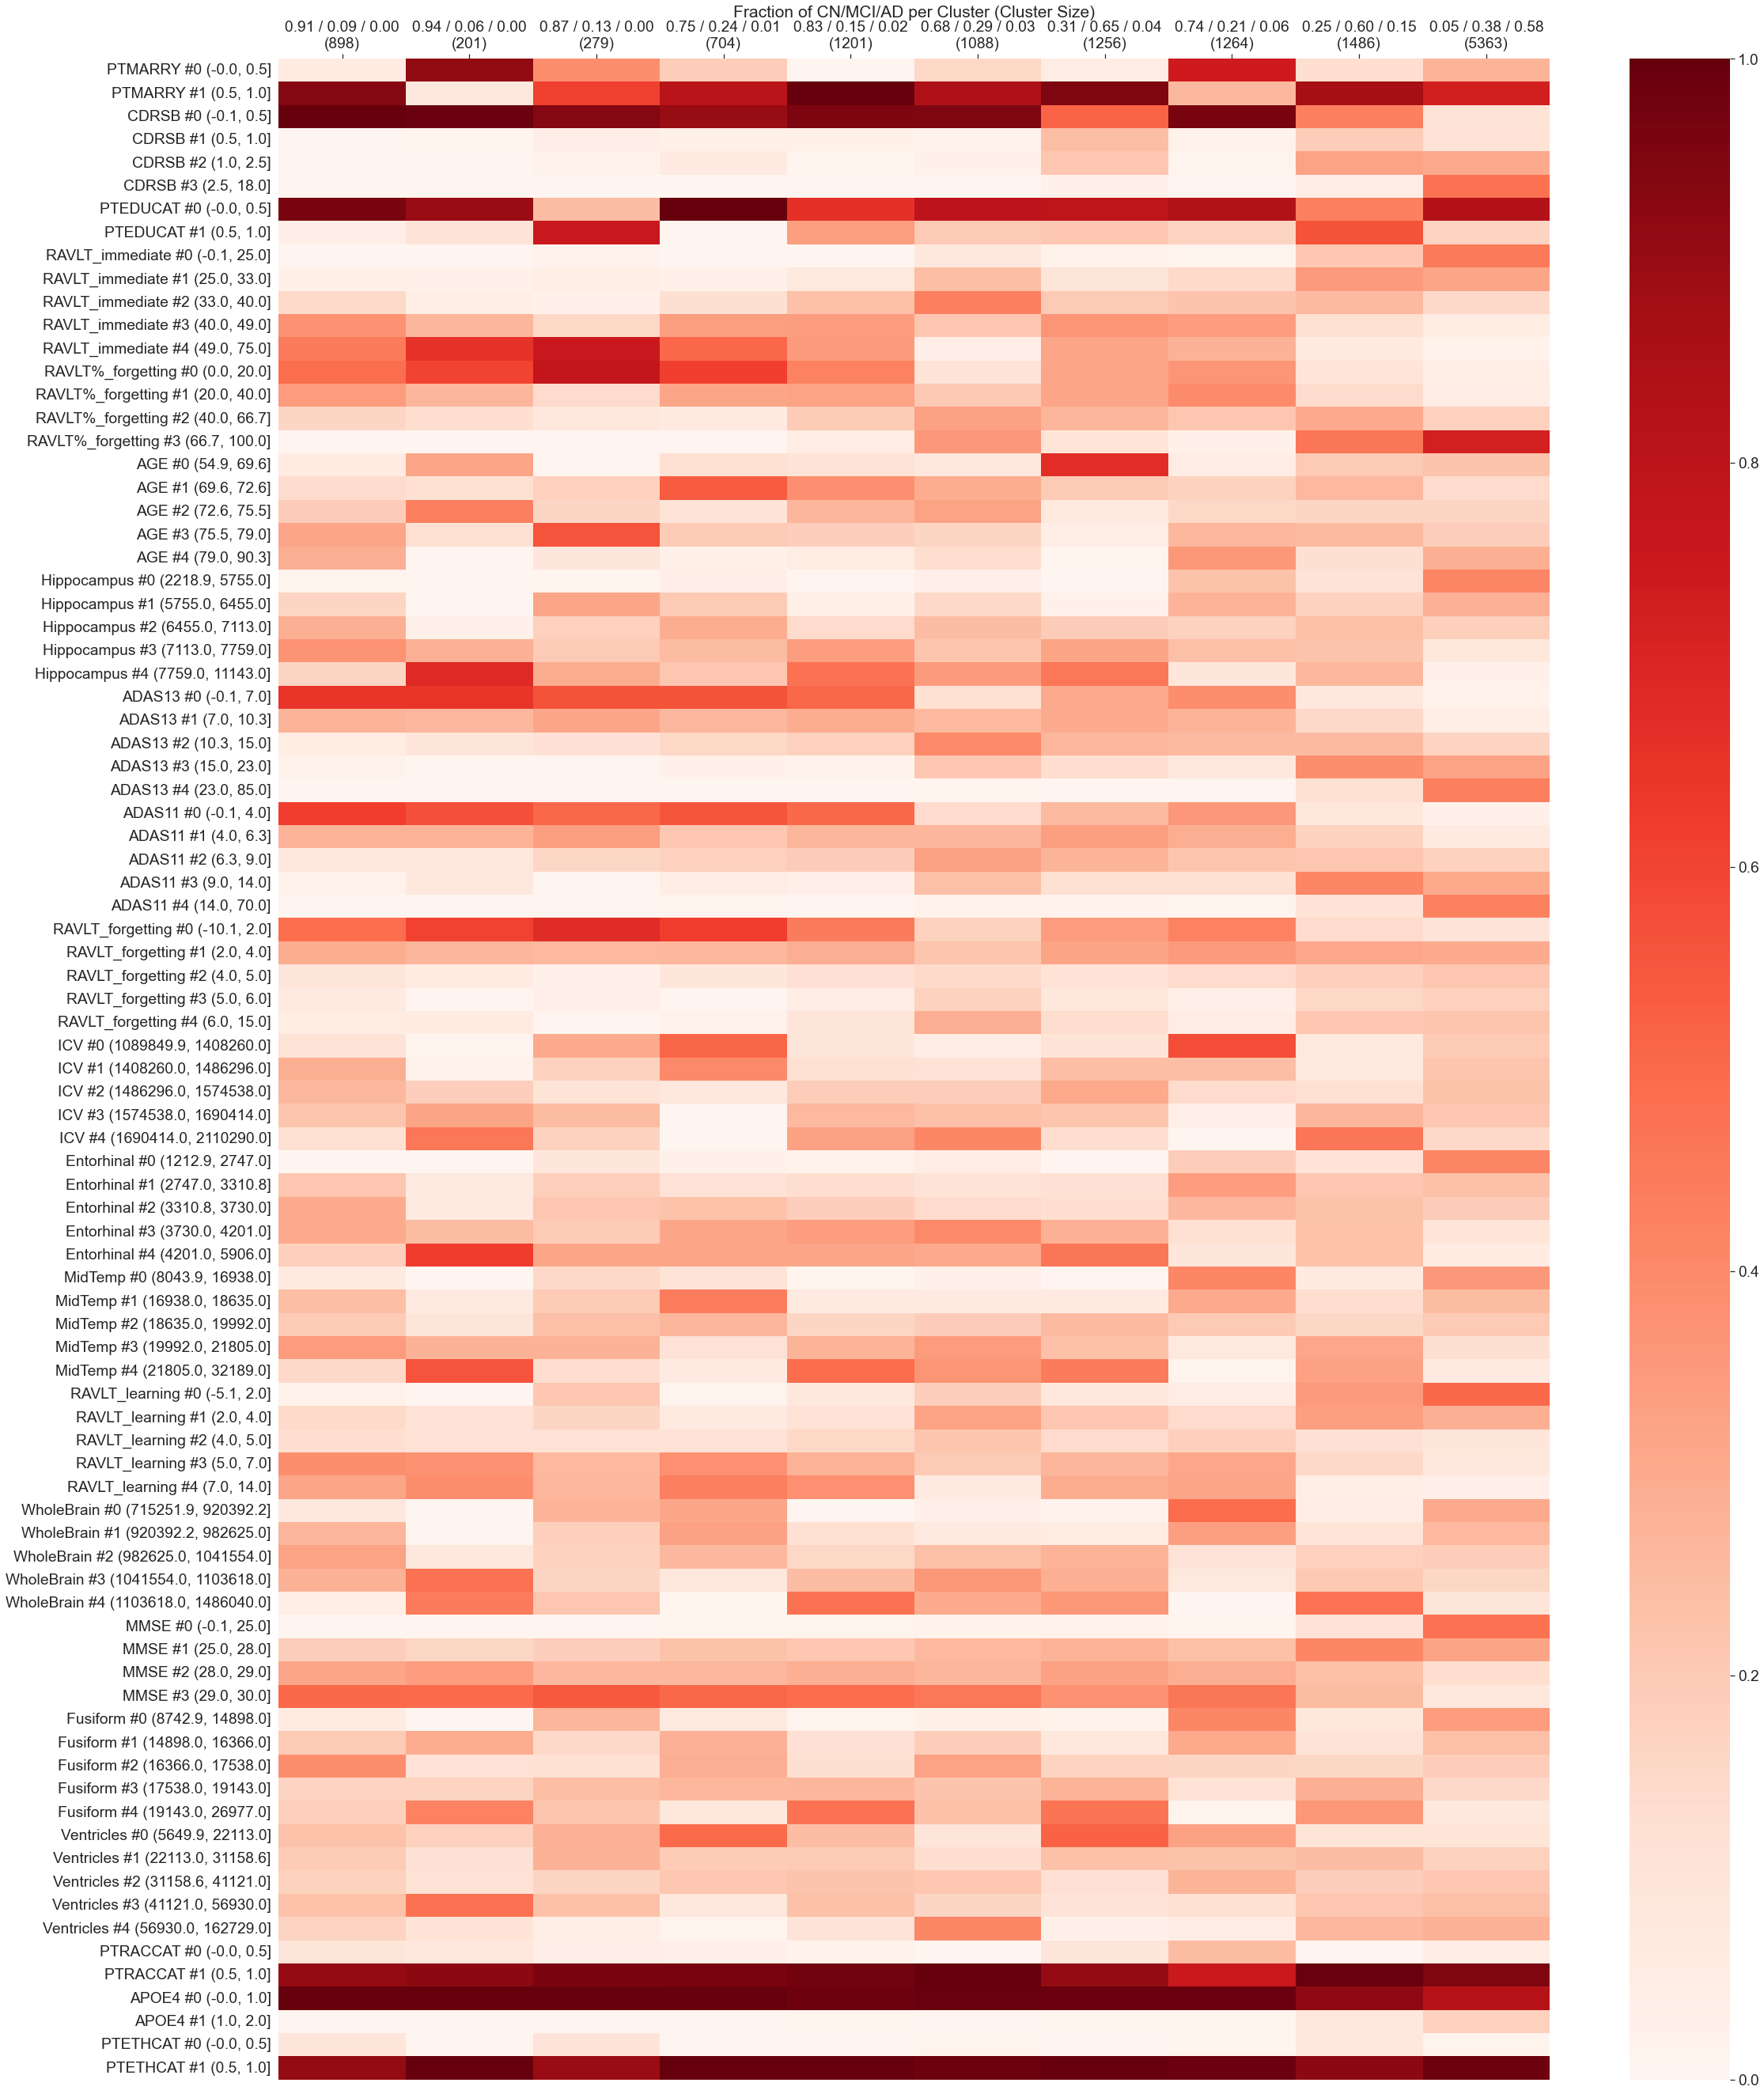
\includegraphics[width=.95\linewidth,height=0.68\textheight,keepaspectratio]{Appendices/appendix-ch02/images/adniHeatmapFull.png}
\centering
  \caption{Heatmap showing how features (rows) vary across clusters (columns) for the ADNI dataset when using \emph{clustering on \ChTwoSmallCaps{Temporal-SCL} learned embedding space}. Heatmap intensity values can be thought of as the conditional probability of seeing a feature value (row) conditioned on being in a cluster (column); these probabilities are estimated using test set snapshots. Columns are ordered left to right in increasing fraction of test set snapshots that come from a time series that has a final outcome of Alzheimer's Disease.
 }
    \ChTwoFloatLabel{ch02:fig:heatmapADNI}  
\end{figure}



% !TeX root = ../../../main.tex
\begin{figure}[t!]
 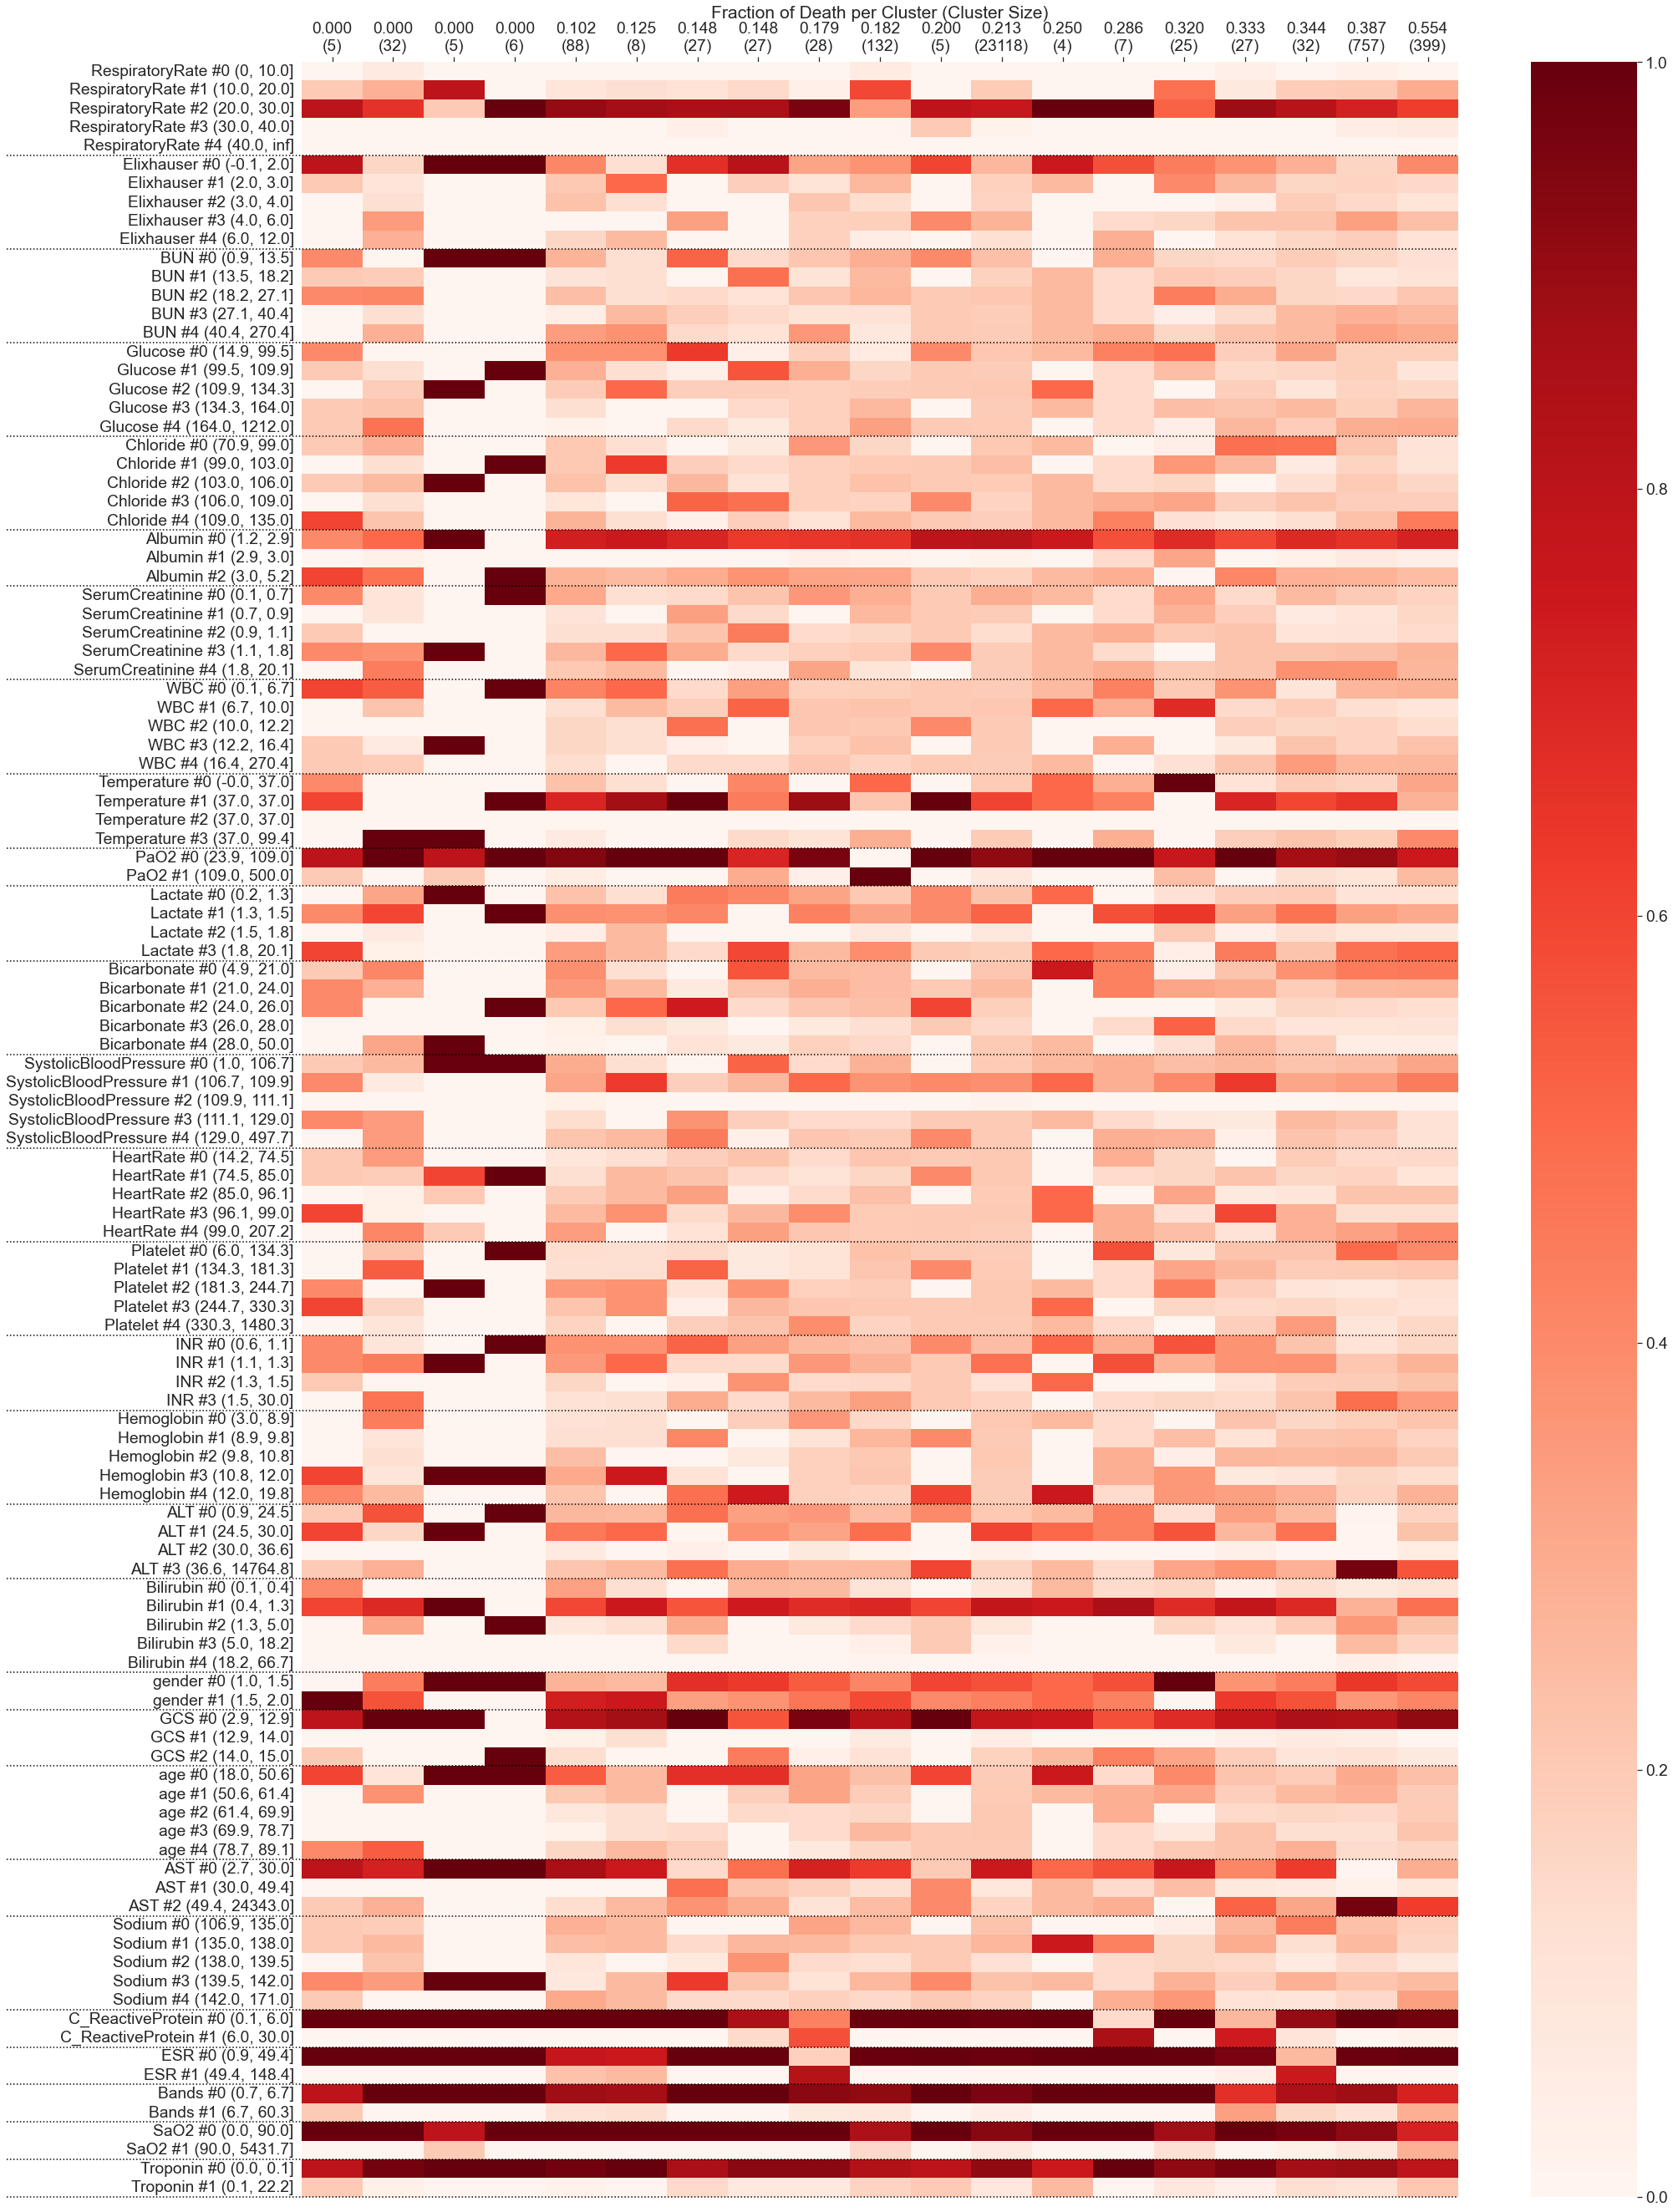
\includegraphics[width=.88\linewidth,height=0.68\textheight,keepaspectratio]{Appendices/appendix-ch02/images/rawMimicHeatmap.png}
\centering
  \caption{Heatmap showing how features (rows) vary across clusters (columns) for the MIMIC dataset when using \emph{clustering on the Raw features} instead of model embeddings. Heatmap intensity values can be thought of as the conditional probability of seeing a feature value (row) conditioned on being in a cluster (column); these probabilities are estimated using test set snapshots. Columns are ordered left to right in increasing fraction of test set snapshots that come from a time series that has a final outcome of death.
 }
    \ChTwoFloatLabel{ch02:fig:RawHeatmapADNI}  
\end{figure}


